%%%%%%%%%%%%%%%
% This bachelor's/master's degree thesis style is based of already applied MS Word template in the 
% Faculty of Electrical Engineering and Electronics of Technical University Gabrovo.
% Author: Svetlozar Kosev
% Last modified: 24 June 2023
%%%%%%%%%%%%%%%

\clearpage
\thispagestyle{empty}


%\thispagestyle{introduction}
%\clearpage
%\thispagestyle{empty}
%\markboth{Въведение}{Introduction}
\addcontentsline{toc}{section}{Въведение}

Сървърът е софтуер/операционна система на устройство, което осигурява услуга на друга програма или потребител. В център за данни (data center), физическата машина, на която се изпълнява програма, често се нарича сървър.
		
		\begin{figure}[h]
			\centering
			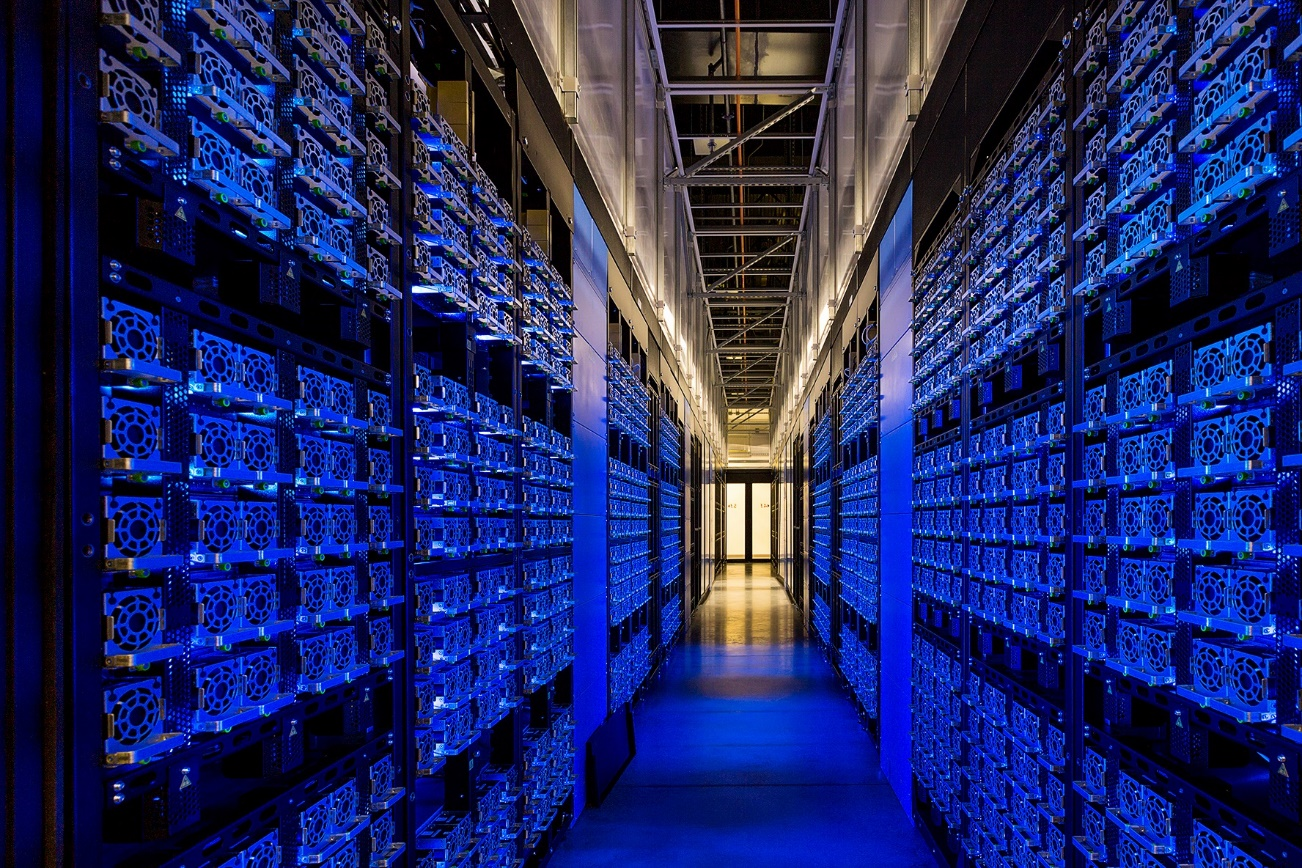
\includegraphics[width=0.8\linewidth]{images/1-1-1Център за данни.png} % replace "example-image" with the filename of your image
			\caption{Център за данни}
			\label{fig:Център за данни}
		\end{figure}
		
		
В моделът клиент-сървър, сървърната програма изчаква и изпълнява заявки от клиентски програми, които могат да се изпълняват в същото време и на други компютри. Някои приложения могат да служат като клиентската програма, с изисквания за услуги, а други – като сървър на заявки от други програми.

Сървърите могат да бъдат както обикновени компютри, така и реално физически или виртуални сървъри със специфичен хардуер и софтуер. Физическия сървър е машина, която се използва за изпълнението на необходим софтуер от клиентите. В повечето случаи, виртуалният сървър е операционна система, инсталирана и конфигурирана с помощта на софтуер за виртуализация. Този тип виртуализация се нарича софтуерна виртуализация (type 2 hypervisor). Популярни софтуери за виртуализация са VirtualBox, VMware Player, KVM, vSphere, QEMU. Изискванията за конфигуриране на виртуализация са процесорът (Intel и AMD) и UEFI/BIOS-ът да я поддържат. (\textit{\textbf{mldunbound.org, 2019}})

		\begin{figure}[h]
	\centering
	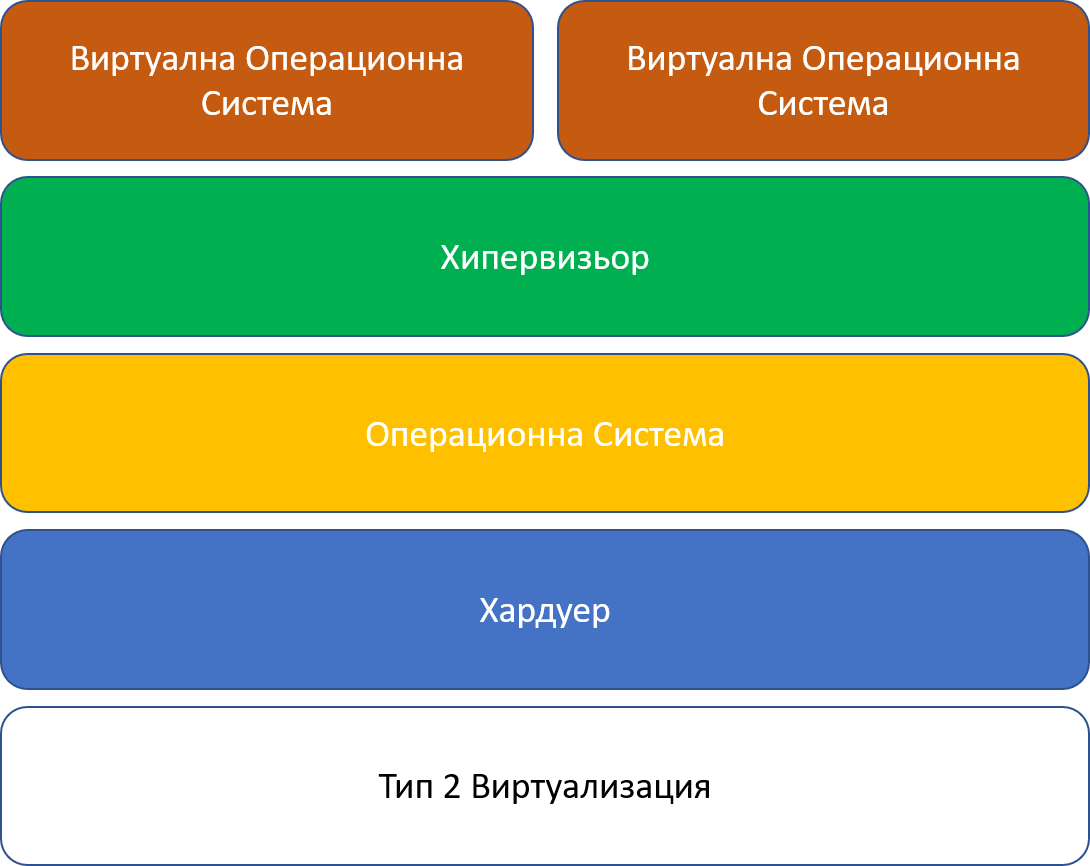
\includegraphics[width=0.8\linewidth]{images/hypervisor2.png} % replace "example-image" with the filename of your image
	\caption{Тип 2 виртуализация}
	\label{fig:Тип 2 виртуализация}
\end{figure}

Другият вид виртуализация е хардуерна (type 1 hypervisor). След като се стартира физическия сървър с инсталиран виртуализатор, се показва екран, приличащ на терминал. Показват се данни за процесора, паметта, мястото за съхранение, IP и MAC адресите. Тук, най-често се използват Hyper-V, Citrix XenServer и VMware ESX.


